\subsection{Introduction}
The electrophysiological signal (acquired from a single electrode) is generally
characterized by two distinct patterns:
\begin{itemize}
    \item \textbf{Spike:} a single over-threshold signal representing the
    electrical activity of a source.
    \item \textbf{Burst:} a sequence of highly packed spikes, often occurring on
    multiple channels at the same time (network burst).
\end{itemize}
Bursting can be defined as a dynamic state with neurons firing discrete groups of
spikes in a repeated manner. A burst is generally followed by a period of quiescence
period. If 2 spikes form a burst are said to be a doublet, 3 are called a triplet,
and so on.
\begin{figure}[H]
    \includegraphics[scale=1.2]{5_1}
    \centering
\end{figure}
Neural bursting plays a key role in communication between neurons, in particular
burst nerons are crucial in mottor pattern generation and synchronization.
Basically all neurons can burst if pharmacologically stimulated, however
it is common to observe autonomous bursting activity, especially in the following
types of neurons:
\begin{itemize}
    \item \textbf{IB:} intrinsically bursting neurons, mostly pyramidal neurons in
    layer 5.
    \item \textbf{CH:} chattering neurons, pyramidal neurons in layers 2, 3, and 4.
    \item \textbf{Interneurons:} present in the cortex.
    \item \textbf{LTB:} low-threshold bursters, they fire high-frequency bursts in
    response to injected pulses of current. Localized in the hippocampus.
    \item \textbf{HTB:} high-threshold bursters fire bursts only in response to
    strong long pulses of current. Localized in the hippocampus.
\end{itemize}
\paragraph{Why do bursts naturally occur?}
There are several hypoteses aiming to explain the importance of bursting activity in
neural computation.
\begin{itemize}
    \item \textbf{Bursts are more reliable than single spikes} in evoking responses in
    postsynaptic cells.
    \item \textbf{Bursts overcome synaptic transmission failure}, it has been shown
    that a synaptic release is more likely to occur in response to a bombardment
    of spikes (instead of a single spike).
    \item \textbf{Bursts evoke long-term potentiation}, thus affecting synaptic
    plasticity in a much greater way than single spikes.
    \item \textbf{Bursts have a higher signal-to-noise ratio} than single spikes, as
    the generation of bursts requires a higher threshold.
    \item \textbf{Bursts encode different features} of sensory input than single
    spikes.
    \item \textbf{Bursts have more informational content} than single spikes, in
    particular when analyzed as unitary events. This information might be encoded
    into the burst duration or in the precise temporal structure of inter spike
    intervals within a burst. 
\end{itemize}
To summarize, it is important to point out that bursts are all-or-none events,
whereas single spikes may be noise.\\
Despite everything, the term burst lack a formal definition, but it is generally employed
to indicate a recording period during which the spiking frequency is especially high,
alternating with periods exhibiting a low spiking frequency (quiescence periods). Therefore,
it can be stated that a burst is characterized by \textbf{small inter spike intervals} and a
\textbf{certain number of spikes}.
\begin{figure}[H]
    \includegraphics[scale=0.25]{5_2}
    \centering
\end{figure}
From a mathematical point of view, a burst can be defined by some properties, such as:
\begin{itemize}
    \item \(t_b\): the starting time of the burst.
    \item \(T_b\): the burst duration.
    \item \(A_b\): the burst amplitude, related to the spike frequency within the burst.
\end{itemize}
The amplitude of a burst is computed as shown below:
\begin{align*}
    A_b=\frac{1}{T_b}\int_{t_b}^{t_b+T_b}\sum_{s=1}^{N}\delta{(t-t_s)}\,dt=\frac{N_{T_b}}{T_b}
\end{align*}
where \(N_{T_b}\) is the number of spikes within the considered burst.
Now, a single-channel burst train \(BT(t)\) can be defined as follow:
\begin{align*}
    BT(t) = \sum_{b=1}^{NB}A_b*\prod\biggl(\frac{t-t_b-\frac{T_b}{2}}{T_b}\biggr)
\end{align*}
with \(NB\) being the number of detected bursts. Notice that the burst train is a sequence
of rectangles. For the multi-channel case (\(M\) channels are considered), the burst train
expression can be easily modified:
\begin{align*}
    BT_{j}(t) = \sum_{b=1}^{NB_{j}}A_b*\prod\biggl(\frac{t-t_b-\frac{T_b}{2}}{T_b}\biggr)
    \quad\quad\text{with}\,j=1,...,M
\end{align*}
Another meaningful way to represent bursts is the burst event train \(BE(t)\), which can
be defined as a point process in which each event corresponds to the starting time of a
burst. It is similar to a spike train, even if the mening is different. Notice that
all the information regarding burst amplitude and duration information are disregarded.
A single-channel burst event train is defined as
\begin{align*}
    BE(t)=\sum_{b=1}^{NB}\delta(t-t_b)
\end{align*}
while in case the channels are multiple \(M\), the definition is simply extended below:
\begin{align*}
    BE_{j}(t)=\sum_{b=1}^{NB_{j}}\delta(t-t_b)
    \quad\quad\text{with}\,j=1,...,M
\end{align*}


\subsection{Burst Detection algorithms}
There are several algorithms aiming at identifying well bursts, some start from raw data,
others require a preprocessing leading to a spike train. The methods presented in the
following belong to this last family, as they are the most spread techniques.

\paragraph{String Method} This algorithm exploits a predefined ISI threshold, set at
\(100\,ms\), representing the maximum inter spike interval such that two subsequent spikes
are considered as part of the same burst. Another important parameter is the minimum
number of spikes required to define as a burst a tightly packed set of spikes. A further
parameter consists in defining a minimum inter burst interval (IBI), thus the minimum time
distance between two candidate bursts to select them as separate events. Notice that
typically the following values are selected:
\begin{itemize}
    \item \(ISI_{max}=100\,ms\)
    \item Minimum number of intra-burst spikes \(=5\)
    \item For simplicity, \(IBI_{min}=ISI_{max}\)
\end{itemize}
This method is of particular interest, as it has a minimal computation footprint, thus
resulting feasible for real-time implementations.

\paragraph{Wagenaar (WA)} The method developed in 2005 by D. A. Wagenaar tries to solve
a problem caused by the fact that usually bursts are characterized by two main parts:
at the beginning (\textbf{burst core}) the spiking frequency is particularly high, while
it tends to become incresingly lower as time passes (\textbf{burst tail}). In order to
better detect the bursts accounting for the differences of the two portions just described,
a system considering two distinct ISI thresholds is employed. The steps carried out
by the algorithm are:
\begin{enumerate}
    \item Set the mean firing rate \(f\), if the signal is multi-channel compute \(f_j\)
    for the \(j\)-th channel.
    \item Define a maximum core ISI, often defined as \(th_{core}=\frac{1}{4f}\)
    or \(th_{core}=100\,ms\).
    \item Look for sequences having at least a minimum number of intra-burst spikes.
    \item Change the maximum ISI threshold to \(th_{tail}=\frac{1}{3f}\) or
    \(th_{tail}=200\,ms\).
    \item Keep looking for spikes before and after the burst core satisfying the
    new threshold condition.
\end{enumerate}

\paragraph{Cocatre-Zilgien and Delcomyn (CZ)} It represents the first method based on the
analysis of the ISI histogram, as it is highly informative about the spiking pattern of
a specific recording channel, as shown in the picture below. In paritcular, bursting
activity tends to result in valleys, due to the fact that two main inter spike intervals
exist, the intra-burst one and the inter-bursts one.
\begin{figure}[H]
    \includegraphics[scale=0.32]{5_3}
    \centering
\end{figure}

\paragraph{Selinger (SE)} This method exploits the ISI histogram (in a logarithmic scale)
to derive the optimal ISI threshold, then it works as a standard single threshold algorithm.
This technique tries to improve the identification of the spikes in the tail portion of a
burst.
\begin{figure}[H]
    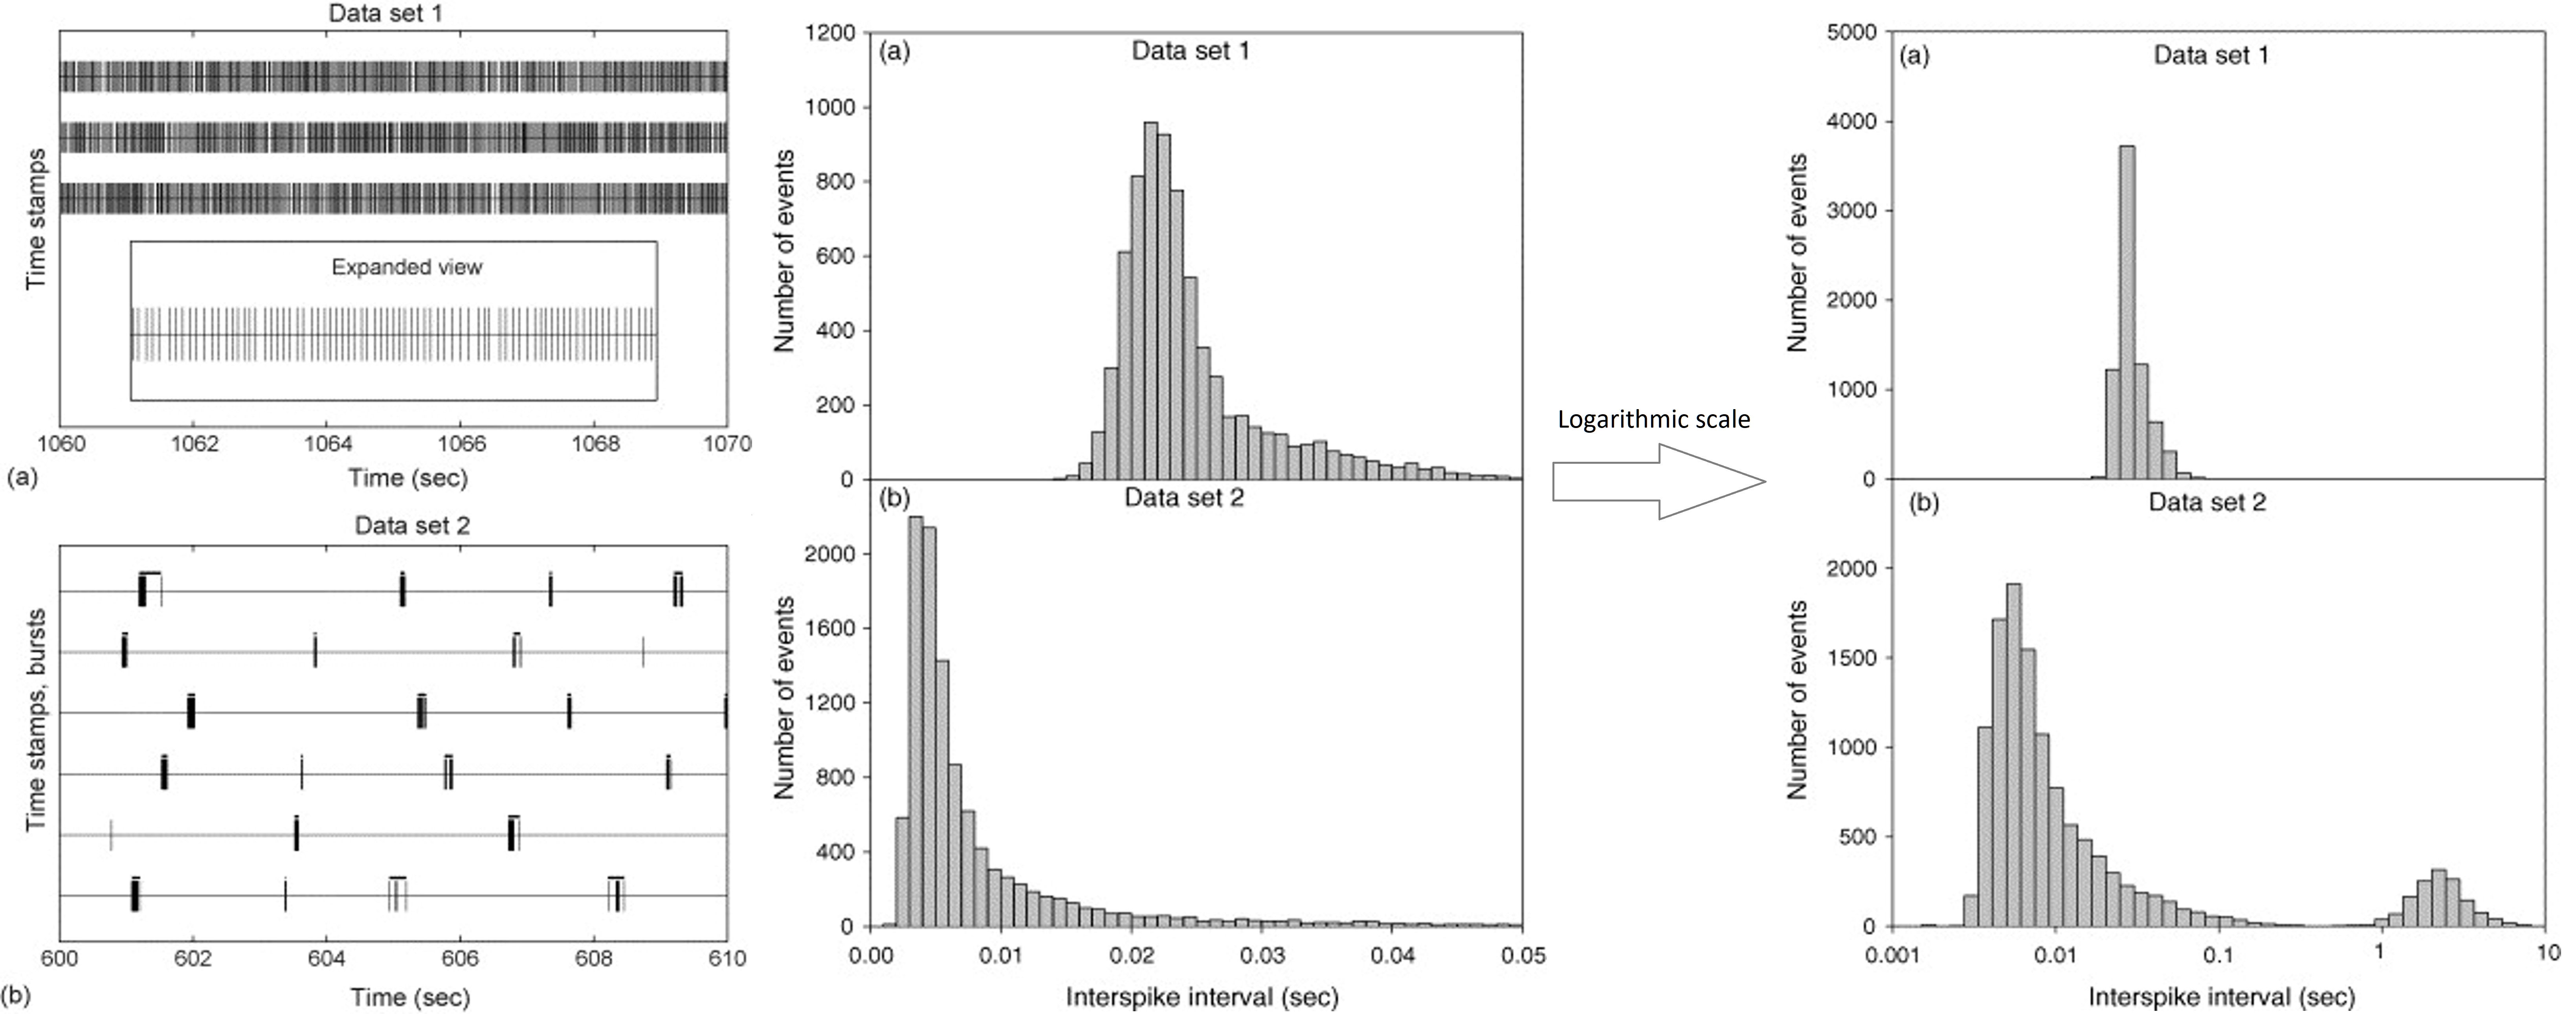
\includegraphics[scale=0.5]{5_4}
    \centering
\end{figure}

\paragraph{Modified Selinger (SE-MOD)} Here it is presented a modified version of the
previously explained Selinger method, consisting in a mix of the already presented
techniques. It allows a better identification of the spikes at the boundaries of a
burst event.
\begin{figure}[H]
    \includegraphics[scale=0.42]{5_5}
    \centering
\end{figure}

Generally, it can be stated that all the implemented burst detection techniques proposed so
far presents pros and cons, thus there is not an algorithm clairly prevailing on the others.
Moreover, different techniques might perform better in different situations, according to
the type of data that are intended to be analyzed.